Algorithm alternatives considered during this research:\\

The stable marriage problem is defined as: Given N men and N women where each man ranks each women from 1 to N and each women ranks men from 1 to N, where 1 is the highest preference and N being the lowest preference. Marriages are one-to-one where one man can only be married to one women and vice versa. Additionally, a marriage is considered unstable if there exist match $\{M_1, W_1\}$ where $M_1$ prefers a another $W_2$ over his current match $W_1$ and $W_2$ prefers $M_1$ over her current match $M_2$. 





\subsection{Parallelization of Gale-Shapley}

The version of Gale-Shapley algorithm chosen to parallelize was the one given by Gusfield et al.\cite{Gusfield:1989:SMP:68392} in 1989. The algorithm is briefly described in Figure \ref{fig:my_label}.

\begin{figure}[h]
    
    \begin{algorithmic}
    \STATE $l \gets $all free men
    \WHILE{some man $m$ in $l$}
        \STATE $w \gets$ woman on $m$'s list to whom $m$ has not yet proposed
        \IF{$w$ is free}
            \STATE assign $m$ and $w$ (they are now engaged)
        \ELSE
            \IF{$w$ prefers $m$ to her fianc\'e $m\prime$} 
                \STATE assign $m$ and $w$, $m\prime$ is now free
            \ELSE
                \STATE $w$ rejects $m$, so $m$ is still free
            \ENDIF
        \ENDIF
    \ENDWHILE
    \end{algorithmic}

    \caption{Gale-Shapley Algorithm as described by Gusfield et al.}
    \label{fig:my_label}
\end{figure}

In order to have a good base line for comparing other algorithms we decide to not change this basic structure of the algorithm. Instead we opted for using concurrent data structures and synchronization mechanisms provided by the language we implemented all of these algorithms, Java. In the implementation section we go in further detail about the chosen concurrent data structures and mechanisms.

In Gale-Shapley algorithm, and man optimal, each women makes at most (men-1) rejections. Additionally the last free women cannot reject a proposal so the maximum number of rejections is (women-1). Assuming (women = men), the maximum number of rejections for all women is $(n-1)*(n-1) = n^2 - 2n +1$ i.e. $O(n^2)$. If we can parallelize rejections in a way that different threads are handling a subsets of rejections, then the performance can be improved. 

\subsection{Stable Marriage by Coroutines}

% OMG just found out that Conway coined the term Coroutine. He is also known by the Conway's Law.
The term coroutine was first explained by Conway in 1963\cite{conway1963design}. A coroutine can be seen as a processing module capable of communicating with other modules through small messages. This communication can happen in both ways, as a coroutine needing some information from another one (input) or producing some information to another coroutine (output). Whenever these messages are passed, control of the program is transferred between coroutines. The main difference between coroutines and threads, from a programmer's point of view, is that for coroutines the programmer decides when to switch to a different executing module occurs. In contrast, threads execution time is decided by the operating system using time slicing and a scheduler, the programmer has no control over it.

In 1983 Allison \cite{allison1983stable} solved the stable marriage problem by using coroutines. The algorithm Allison was based on McVitie and Wilson's algorithm \cite{mcvitie1971stable}, where each man proposes to each of the woman in his preference list until he is accepted. A man can propose to a woman and the woman could be either free or engaged. If the woman is free, she immediately accepts, or engaged, in this case she evaluates the proposal and jilts her worst choice. The algorithm continues until all men and women are matched. Allison provides an implementation of the algorithm in the language Modula-2\footnote{https://www.modula2.org/reference/index.php}.\\
In the provided implementation by Allison, there is a main program that creates coroutine instances for every man and every woman. An instance of a man coroutine simply loops over his list of preferences and transfers control of execution to every woman coroutine in order. This is a man proposing to a woman. Once the preferred woman coroutine gains control it evaluates if it is free, if so she accepts and transfer control to the main program, if not then compares ranking in its list of preferences and transfers control to the less preferred man coroutine. Finally, the main program simply transfers control to each man coroutine until all of them are married. 

\subsection{Stable Marriage Problem by Divide-and-Conquer Approach}

Divide and conquer approach was discussed in \cite{tseng1984parallel}. This approach divides the problem into smaller subsets where each subset can be resolved in isolation from other subsets allowing things to be parallelized. For example:
Given the preference list in Figure \ref{fig:parallel_example_case}, initially, in a man optimal matching, each man will be matched with their first preference. Once we have the initial pair the problem can be broken down into four separate subsets or pair. 
Initial Pairs:

\begin{figure}[!ht]
    \centering
    
    \begin{tabular}{lllllllllllll}
$M_1$ & 3     & 2    & 1    & 4       &  & $W_1$ & 1     & 3     & 2     & 4  \\
$M_2$ & 3     & 1    & 2    & 4       &  & $W_2$ & 4     & 1     & 3     & 2  \\
$M_3$ & 4     & 3    & 1    & 2       &  & $W_3$ & 4     & 3     & 1     & 2  \\
$M_4$ & 2     & 4    & 3    & 1       &  & $W_4$ & 2     & 4     & 3    & 1 \\
   & \multicolumn{4}{l}{Men's ranking} &  &    & \multicolumn{4}{l}{Women's Ranking}
\end{tabular}
    
    \caption{Example Preference List $n=4$}
    \label{fig:parallel_example_case}
\end{figure}

\begin{figure}[!ht]
    \centering
    
    \begin{tabular}{lllllllllllll}
Pair1 & (M1, W3)  \\
Pair2 & (M2, W3)  \\
Pair3 & (M3, W4)  \\
Pair4 & (M4, W2)  \\
\end{tabular}
    
    \caption{Initial Pairs}
    \label{fig:Initial Pairs}
\end{figure}

After getting the initial pairs, we then start the merging process.Each subset, a set of 2 pairs in this case, will then be merged with another subset effectively reducing it to one matching. Once the merged set is constructed, we need to make sure that the matching in the subset is stable i.e. no woman is match to more than one man. If no woman is match to two men then we know that matching is stable since both men got their first choice and no woman was repeated. However, if a woman is matched to two men as in the case above {(M1, W3), (M2, W3)}, then we have to check the women preference list and choose the man she favors. Once we know which man the women favors, then we can advance the other man into his next women on his preference list. This logic will happen iteratively as the subsets merge and grow. Each merged subset will effectively result in a stable matching. At the very end there will be two big subsets that when merged together will result in final optimal stable matching result. Each merge of two subsets can happen in parallel in different threads. The problem starts with n pairs and then divides by two iteratively until we end up with 1 subset.

\begin{figure}[!ht]
    \centering
    \scalebox{.3}{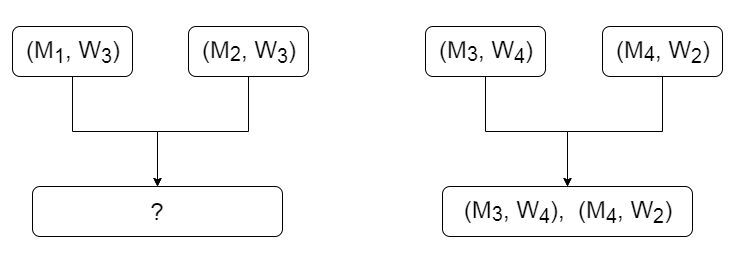
\includegraphics{figures/DivideAndConquer_1.png}}
    \caption{First Merge - Conflict}
    \label{fig:DivideAndConquer_1}
\end{figure}

\begin{figure}[!ht]
    \centering
    \scalebox{.3}{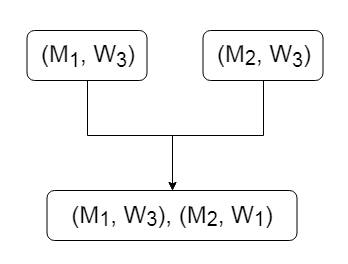
\includegraphics{figures/DivideAndConquer_3.png}}
    \caption{First Merge- Conflict Resolved}
    \label{fig:DivideAndConquer_1}
\end{figure}

\begin{figure}[!ht]
    \centering
    \scalebox{.3}{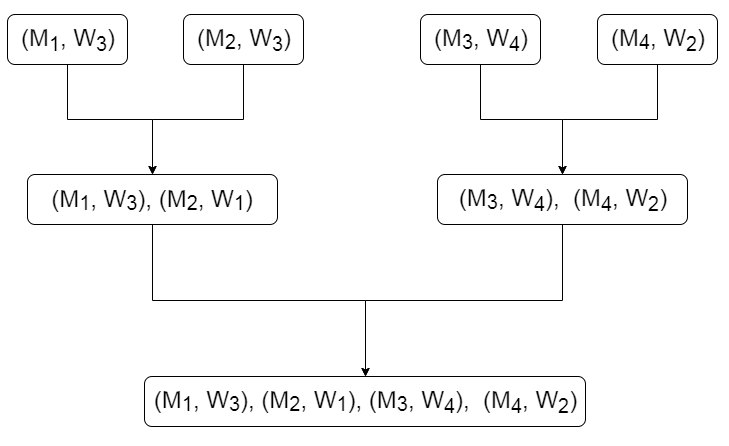
\includegraphics{figures/DivideAndConquer_2.png}}
    \caption{Final Matching}
    \label{fig:DivideAndConquer_1}
\end{figure}




\subsection{Master-Slave Implementation}
The Master-Slave approach to the Gale-Shapely algorithm was based on a model where a master controls all communication between men and women.\cite{larsen1997parallel} The basic algorithm can be thought of in two parts:
\begin{enumerate}
    \item Proposal phase - the master presents all the open proposals to all those receiving proposal requests.
    \item Response phase - in parallel, the ones accepting requests decide the preferred one and return the rejected requests to the master
\end{enumerate}
This process repeats until all matches have been assigned. When evaluating proposals, the master groups proposals together. The slaves are therefor not responding to proposals to one at a time, but as a group. For instance, if a, b, and c all desire x. The master will send all three proposals and x will decide between the three of them right then and there. This is done in a series of rounds so all of the proposer's first preference gets gathered up by the master and sent out. After matches are assigned, all of the proposers who are unassigned have their second preference gathered up and sent out. If a proposer is assigned a match and then rejected, they pick up right where they left off in their proposal position regardless of where their fellow proposers are.


\subsection{Parallel Iterative Improvement Stable Matching Algorithm} Enyue et. al\cite{PII} present a solution for the stable matching problem that deviates considerably from the approach introduced with Gale-Shapley introduced. The approach they published is called Parallel Iterative Improvement (PII) algorithm, and revolves around a ranking matrix built with the preferences of both men and women. The algorithm claims to execute at its best when run on $n^2$ processors.
\subsubsection{Creation of Ranking Matrix}
Figure \ref{fig:PII Ranking Matrix} shows how the initial setting for the PII algorithm is composed. Taking into account a set of preferences for both men and women, a matrix is formed with each field containing a pair build by mixing the preference of a man and a woman. In order to keep a geometrical co-relation between coordinates and matching participants. rows are assigned to men and columns represent women preferences. Men preferences are placed as the left value for each field, whereas women preferences are placed on the right of each field, with the arrangement of preference values being transposed, as each column represents the preference list of a woman.

\begin{figure}[!ht]
    \centering

    \begin{tabular}{lllllllllllllll}
   & \multicolumn{4}{l}{Men's ranking} &  \multicolumn{4}{l}{Women's Ranking}\\
$M_1$ & 4    & 2    & 3    & 1    & $W_1$ & 1     & 4     & 2   & 3 \\
$M_2$ & 3    & 2    & 1    & 4    & $W_2$ & 1     & 2     & 3   & 4  \\
$M_3$ & 2    & 4    & 1    & 3   & $W_3$ & 4     & 2     & 3     & 1  \\
$M_4$ & 1    & 4    & 3    & 2    & $W_4$ & 3     & 1     & 4     & 2 \\
\\

& & &&\multicolumn{3}{l}{Ranking Matrix}\\
 & & & 4,1 & 2,1 & 3,4 & 1,3\\
 &&& 3,4 & 1,2 & 2,2 & 4,1\\
 &&& 2,2 & 4,3 & 1,3 & 3,4\\
 &&& 1,3 & 4,4 & 3,1 & 2,2\\
\end{tabular}\\

    \caption{PII Preference Matrix $n=4$}
    \label{fig:PII Ranking Matrix}
\end{figure}

\subsubsection{Initial Matching}
Initial matching values are assigned randomly. A matching set with the presented matrix configuration has the form of a set of pairs, called \textit{matching pairs}, representing the engagement between the man linked to the row coordinate and the woman linked to the column coordinate. As each matching member can only be matched once, there can only be one matching pair per row and column. The random assignment of initial matching pairs is done via the Random Permutation Algorithm. \cite{Durstenfeld}.
\subsubsection{Iteration Phase}
The most complex part of the algorithm. It consists on the identification of unstable pairs, which are what are normally regarded as blocking pairs. the process of identification requires each pair in the matrix to be compared against the matches on their same row and column, if both preferences in a given pair are higher than the one for the man(left element in the matching pair on the same row) and woman (right element of the matching pair in the same column).\\
Once unstable pairs are identified, two different sets of pairs $NM_1$ and $NM_2$ are computed as described in \cite{PII}. The union of these two values represent the elements to be used in a new matching set, which is completed by adding the initial matching without any pairs in the rows and columns that the new matching pairs are located on.\\
After a new matching set is calculated, all the steps described for the iteration phase are repeated until there are no unstable pairs found. When the different steps in the iteration phase are paralleled, there is a possibility for loops to be generated, where the new matching calculated will have a repeating pattern. One measure to be take in order for this misbehavior to be mitigated is limiting number of times the iterations phase may be executed, and recalculating a Random Permutation initial matching again, starting a new iteration phase with it.